% 
\section{Introduction}
\label{methodology:introduction}
%
The methodology outlines the systematic approach taken to conduct the research. It provides a detailed account of the research design, data collection methods, and analysis techniques employed. The rules for this section emphasize clarity and reproducibility. The methodology must be described in a step-by-step manner, enabling other researchers to replicate the study. It should justify the chosen methods, explaining how they align with the research questions and objectives. Precision is crucial; each method and tool used must be clearly defined. Additionally, ethical considerations and limitations should be addressed, ensuring transparency and integrity in the research process.

Provide a visual representation of the comprehensive proposed methodology, and elaborate on it. For instance, refer to Fig. \ref{figure:methodology} for an illustrative example\footnote{https://techsparks.co.in/hot-topic-for-project-and-thesis-machine-learning/} of the methodology in action.

\begin{figure}[H]
\centering
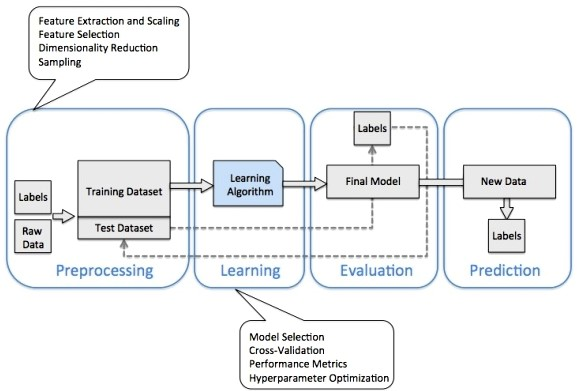
\includegraphics[scale=2.5]{methodology}
\caption{Proposed Methodology}
\label{figure:methodology}
\end{figure}


%
\section{Section(s)}
\label{methodology:section}
%
To provide a comprehensive understanding of the proposed methodology, break it down into easily digestible sections and subsections. Thoroughly explain each component and model selection, emphasizing the rationale behind the choices. Ensure clarity and accessibility throughout the document, making it easy for readers to grasp the presented concepts. Additionally, maintain proper citation practices, giving due credit when incorporating external resources, such as images or data, into the work.

You can generate an abbreviation and incorporate it into your text, for example: \gls{hstu}. Upon initial use, the complete meaning will be displayed. Subsequent references will only present the abbreviated form, such as \gls{hstu}.

Here are some examples of lists (bullet and numbered), tables, algorithms, and equations.

The following list consists of unordered bullet points.

\begin{itemize} \label{asd}
    \item \textbf{Label 1:} Some text...
    \item \textbf{Label 2:} Some text...
\end{itemize}

The following list consists of numbered points.

\begin{enumerate}
    \item \textbf{Label A:} Some text...
    \item \textbf{Label B:} Some text...
\end{enumerate}

Table \ref{table:results} displays randomly generated values for accuracy, precision, and F1-score as performance measures.

\begin{table}[H]
\centering
\caption{Results of Experiment}
\label{table:results}
\begin{tabularx}{0.8\linewidth}{@{ } X | *{3}{r} @{ }}
\toprule
\multirow{2}{*}{Model} & \multicolumn{3}{c}{Dataset} \\ 
        & Accuracy             & Precision              & F1      \\ 
\midrule
Model A & {93.57}  & {77.24}  & {95.36}           \\ 
Model B & {95.70}  & {60.51}  & {73.67}           \\ 
Model C & {56.46}  & {30.16}  & {54.47}           \\ 
Model D & {73.91}  & {37.70}  & {71.03}           \\ 
Model E & \textbf{98.41}  & \textbf{44.28}  & \textbf{76.91}  \\ 
Model F & {87.73}  & {43.17}  & {75.79}           \\
\bottomrule
\end{tabularx}
\end{table}

Algorithm \ref{algorithm:dividenumber} shows the steps for division of two numbers.

\begin{algorithm}[H]
\caption{ Divide Number ($num1, num2$)}
\label{algorithm:dividenumber}
\begin{algorithmic}[1]
\If{$num2 = 0$}
    \State return $Unknown$
\EndIf
\State $result = num1 / num2$
\State return $result$
\end{algorithmic}
\end{algorithm}

Equations (\ref{eq:one}) to (\ref{eq:three}) demonstrate the usage of the align construct for defining multiple equations.

\begin{align}
    (w^T x_i-\gamma)>=+1    \label{eq:one} \\
    (w^T x_i-\gamma)<=-1    \label{eq:two} \\
    (w^T x_i-\gamma)=0      \label{eq:three}
\end{align}

The formula for accuracy metric is given in (\ref{eq:accuracy}), where True Positives (\textit{TP}) are the correctly predicted positive cases, True Negatives (\textit{TN}) are the correctly predicted negative cases, False Positives (\textit{FP}) are the incorrectly predicted positive cases and False Negatives (\textit{FN}) are the incorrectly predicted negative cases.

\begin{equation}
\label{eq:accuracy}
accuracy = \frac{TP + TN}{TP + FP + TN + FN}
\end{equation}

\bigskip
You can also write in other languages by defining new font faces and uploading the \textit{ttf} file. For example, the following line is in Bengali: {\myfont{আমাদের সবাই একসাথে আগামী ভবিষ্যতের দিকে যাচ্ছি}}.

